\documentclass{article}
\usepackage[sexy, hdr, fancy]{evan}
\usepackage{graphicx}
\setlength{\droptitle}{-4em}

\lhead{Homework 1}
\rhead{Introduction to Statistics}
\lfoot{}
\cfoot{\thepage}

\begin{document}
\title{Homework 1}
\maketitle
\thispagestyle{fancy}

\begin{enumerate}

		%% Problem 1
		\ii Recall that a random variable is exponentially distributed with parameter $\lambda$ if its density function $f(x)$ is given by \[f(x) = \lambda e^{-\lambda x} \text{ for } x\text{ positive, and 0 otherwise.} \]
			
		\begin{enumerate}[(a)]
				\ii Suppose a random variable $T$ has a Weibull $(\lambda, \alpha)$ distribution, i.e. that $T$ has density \[f(t) = \lambda\alpha t^{\alpha-1}e^{-\lambda t^{\alpha}}\] for $t>0, \lambda>0, \alpha>0.$ Show that $T^{a}$ has exponential $(\lambda)$ distribution.
				\begin{proof}
					We use the fact that \[\frac{d}{dx}F_X(x) = f_X(x)\] where $F_X(x)$ is the cumulative distribution function, that is, \[F_X(x) = P(X\le x) = \int_{-\infty}^x f(t)\, dt.\] Thus to determine the distribution of $T^\alpha$ we may compute the CDF of $T^\alpha$ and take the derivative with respect to $x.$ 
					The probability we desire is \[P(T^\alpha\le x) = P(T\le x^{1/\alpha})\] where we used the fact that $T^\alpha$ is convex for $\alpha>0.$ We know the distribution of $T$, so this probability is \[F_T(x^{1/\alpha}) = \int_{-\infty}^{x^{1/\alpha}} \lambda\alpha t^{\alpha-1}e^{-\lambda t^{\alpha}}\, dt.\] Taking the derivative of both sides with respect to $x$ and invoking the chain rule, we have \begin{align*}
						\frac{d}{dx}F_T(x^{1/\alpha}) &= \left( \frac{d}{dx}x^{1/\alpha} \right) \lambda\alpha (x^{1/\alpha})^{\alpha-1}e^{-\lambda (x^{1/\alpha})^{\alpha}} \\
						&= \left(\frac{1}{\alpha}x^{\frac{1-\alpha}{\alpha}} \right) \lambda\alpha x^{\frac{\alpha-1}{\alpha}}e^{-\lambda x} \\
						&= \lambda e^{-\lambda x}.
					\end{align*}

					Thus the distribution for $T^\alpha$ is the exponential distribution with parameter $\lambda,$ as desired.
				\end{proof}

				\newpage

				\ii Show that if $U$ is a uniform (0, 1) random variable, then $T=(-\lambda^{-1} \log U)^{1/\alpha}$ has a Weibull $(\lambda, \alpha)$ distribution.

				\begin{proof}
					We proceed with the same approach as the previous part, where we calculate the CDF of $T,$ then take its first derivative to determine its PDF.
					\begin{align*}
						P(T\le t) &= P\left[ \left( -\frac{1}{\lambda}\log U \right) \le t \right] \\
						&= P\left( -\frac{1}{\lambda}\log U \le t^\alpha \right) \\
						&= P\left( \log U\ge-\lambda t^\alpha \right) \\
						&= P\left( U\ge e^{-\lambda t^\alpha} \right)
					\end{align*}

					Since $U$ is a uniform (0, 1) variable, this probability is equal to $1-e^{-\lambda t^\alpha}.$ To finish, note that \[f_T(t)=\frac{d}{dt}P(T\le t) = \frac{d}{dt}\left( 1-e^{\lambda t^\alpha} \right) = 	\lambda\alpha t^{\alpha-1}e^{-\lambda t^{\alpha}}, \] which is the desired distribution.		
				
				\end{proof}

				\ii Let $X_1, X_2, \cdots, X_n$ be i.i.d exponential $\lambda$ random variables. Calculate the distribution of their sum $T_n=\sum_{i=1}^n X_i.$

				\begin{proof}
					We will show that the density distribution of $T_n$ is given by \[g_n(t) = \frac{(\lambda t)^{n-1}}{(n-1)!}\lambda e^{-\lambda t}. \] We proceed by induction. The base case $n=1$ is trivial, \[g_1(t)=\frac{(\lambda t)^{1-1}}{(1-1)!}\lambda e^{\lambda t} = \lambda e^{-\lambda t}, \] which is the distribution for $X_1.$ Next, assume that \[g_k(t) =  \frac{(\lambda t)^{k-1}}{(k-1)!}\lambda e^{-\lambda t}\] for arbitrary $k>1.$ We wish to determine the density $h(t)$ for $T_{k+1}=T_k+X_{k+1},$ which we can do via convolution of the two random variables. Let $f(x)$ be the density for $X_{k+1},$ which is an exponential variable. We have  
					
					\begin{align*}
						h(t) &= \int_0^t g_k(x) f(t-x)\, dx \\
						&= \int_0^t \frac{(\lambda x)^{k-1}}{(k-1)!}\lambda e^{-\lambda x} \cdot \lambda e^{-\lambda(t-x)}\, dx \\
						&= \frac{\lambda^{k+1}e^{-\lambda t}}{(k-1)!}\int_0^t x^{k-1}\, dx \\
						&= \frac{\lambda^{k+1}e^{-\lambda t}}{(k-1)!}\left( \frac{1}{k}x^k \right)\Bigg|_0^t \\
						&= \frac{\lambda^k t^k}{k!}\lambda e^{-\lambda t} = g_{k+1}(t),
					\end{align*} thus $h(t)=g_{k+1}(t),$ so the inductive hypothesis is true and we are done.

				\end{proof}

				\ii Show that this is a special case of the more general \textit{gamma distribution with parameters} $\alpha$ \textit{and} $\beta,$ whose density $f(x)$ is given by \[ f(x) = \frac{x^{\alpha-1}e^{-x/\beta}}{\beta^\alpha\Gamma(\alpha)}, \quad\text{for } x>0 \] where $\Gamma(\alpha)=\int_0^\infty t^{\alpha-1}e^{-t}\, dt.$
				\begin{proof}
					Let $\alpha=k$ and $\beta=1/\lambda.$ If $k\in\ZZ^+,$ we have $\Gamma(k)=(k-1)!$ (this is true in our special case, since $k$ indexes the $X_i$). Thus, we have \[f(x)=\frac{x^{k-1}e^{-\lambda x}}{(1/\lambda)^k(k-1)!} = \frac{(\lambda x)^{k-1}}{(k-1)!}\lambda e^{-\lambda x}, \] as desired.
				\end{proof}

		\end{enumerate}

	\newpage

	%% Problem 2
	\ii Let $X_i$ be i.i.d uniform [1, 2] random variables. 
		
	\begin{enumerate}[(a)]
		\ii Compute the expectation $\mu$ and the variance $\sigma^2$ of the random variables $R_i=\ln X_i.$ 

		\begin{soln}
			Since $X_i$ are uniform [1, 2] random variables, the density distribution is identically 1 on its domain. Then \[E[R_i] = \int_1^2 \ln x\, dx = (x\ln x-x)\bigg|_1^2 = \boxed{2\ln 2 - 1,} \] where we integrated by parts to determine the integral of $\ln x.$
			Next, $var(R_i)=E[R_i^2]-(E[R_i])^2,$ so we are interested in $E[R_i^2].$ This is \[\int_1^2 (\ln x)^2\, dx. \] We integrate by parts using $u=\ln x, du = 1/x, dv = \ln x\, dx, v = x\ln x-x,$ and the integral evaluates to 
			\begin{align*}
				\int_1^2 (\ln x)^2\, dx &= \left( x(\ln x)^2 - x\ln x \right)\bigg|_1^2 - \int_1^2\ln x - 1\, dx \\
				&= \left( x(\ln x)^2-x\ln x - (x\ln x - x - x) \right)\bigg|_1^2 \\
				&= \left( x(\ln x)^2 -2x\ln x + 2x \right)\bigg|_1^2 \\
				&= 2(\ln2)^2 - 4\ln2 + 2
			\end{align*}

			Thus 
			\begin{align*}
				var(R_i) &= E[R_i^2]-(E[R_i])^2 \\
				&= 2(\ln2)^2-4\ln2+2-(2\ln2-1)^2 \\
				&= \boxed{1-2(\ln2)^2.}
			\end{align*}
		\end{soln}

		\ii Let $Y_n$ be the random variable \[Y_n = (X_1X_2\cdots X_n)^{1/n}. \] Determine what happens of $Y_n$ as $n\to\infty;$ if it converges, specify its limiting distribution; and if not, explain why.

		\begin{soln}
			To begin, note that $Y_n$ is bounded between the values 1 and 2, thus it converges.

			Consider the random variable \[Z_n=\ln Y_n=\ln\left( \prod_{i=1}^n X_i \right)^{1/n} = \frac{1}{n}\sum_{i=1}^n \ln X_i. \] Thus as $n\to\infty,$ the distribution of $Z_n$ approaches a normal distribution with 
			\begin{align*}
				\mu &= E[\ln X_i] = 2\ln 2-1 \\
				\sigma^2 &= \frac{var(\ln X_i)}{n} = \frac{1-2(\ln2)^2}{n}.
			\end{align*}

			Thus \[\ln Y_n \sim N\left( 2\ln 2-1, \frac{1-2(\ln2)^2}{n} \right) \]

			so $Y_n$ is limited by the log-normal distribution with the above parameters.
			
		\end{soln}
	\end{enumerate}
	
	\newpage

	%% Problem 3
	\ii Suppose the pair $(X_1, X_2)$ has a bivariate normal distribution with parameters $(\mu_1, \mu_2, \sigma_1^2, \sigma_2^2, \rho)$ where $|\rho|<1;$ that is, the bivariate density is given by \[f_{X_1, X_2}(x_1, x_2) = \frac{\exp{(-A(x_1, x_2)/2)}}{2\pi\sigma_1\sigma_2\sqrt{1-\rho^2}}\] and $A(x_1, x_2)$ is defined as \[A(x_1, x_2) = \left[\left( \frac{1}{1-\rho^2} \right) \left(\frac{(x_1-\mu_1)^2}{\sigma_1^2}-2\rho\frac{(x_1-\mu_1)(x_2-\mu_2)}{\sigma_1\sigma_2}+\frac{(x_2-\mu_2)^2}{\sigma_2^2}\right) \right]. \]
	
	\begin{enumerate}
			\ii Let $\vec{x}$ denote the row vector $\vec{x}=\begin{bmatrix}
				x_1 & x_2
			\end{bmatrix},$ and let $\mu$ denote the row vector of means $\mu=\begin{bmatrix}
				\mu_1 & \mu_2
			\end{bmatrix}.$ Let $\Sigma$ denote the matrix of covariances, so $\Sigma_{ij}=cov(X_i, X_j).$ Show that the bivariate density above can be equivalently expressed as \[f_{X_1, X_2}(x_1, x_2) = \frac{\exp{(-A(x_1, x_2)/2)}}{C}\] where $C$ is a constant, and $A(x_1, x_2)$ is the \textit{quadratic form} defined by \[A(x_1, x_2)=(\vec{x}-\mu)\Sigma^{-1}(\vec{x}-\mu)^{T}\] and \[\rho=\frac{cov(X_1, X_2)}{\sigma_1\sigma_2} \text { is the so-called \it{correlation} between } X_1 \text{ and } X_2. \] Express the constant $C$ in terms of the determinant of $\Sigma.$
				\begin{proof}
					We have
					\begin{align*}
						\Sigma&=\begin{bmatrix}
							cov(X_1, X_1) & cov(X_1, X_2) \\
							cov(X_2, X_1) & cov(X_2, X_2)
						\end{bmatrix} = \begin{bmatrix}
							\sigma_1^2 & \rho\sigma_1\sigma_2 \\
							\rho\sigma_1\sigma_2 & \sigma_2^2
						\end{bmatrix} \\
						\det{\Sigma} &= \sigma_1^2\sigma_2^2(1-\rho^2) \\
						\implies \Sigma^{-1} &= \frac{1}{\sigma_1^2\sigma_2^2(1-\rho^2)}\begin{bmatrix}
							\sigma_2^2 & -\rho\sigma_1\sigma_2 \\
							-\rho\sigma_1\sigma_2 & \sigma_1^2
						\end{bmatrix}
					\end{align*}

					Then \[(\vec{x}-\mu)=\begin{bmatrix}
							x_1-\mu_1 & x_2-\mu_2
						\end{bmatrix}, \quad\quad (\vec{x}-\mu)^{T} = \begin{bmatrix}
							x_1-\mu_1 \\ x_2 - \mu_2
					\end{bmatrix}\] so 
					\begin{align*}
						(\vec{x}-\mu)\Sigma^{-1}(\vec{x}-\mu)^T &= \begin{bmatrix}
							x_1-\mu_1 & x_2-\mu_2
						\end{bmatrix} \cdot \frac{1}{\sigma_1^2\sigma_2^2(1-\rho^2)}\begin{bmatrix}
							\sigma_2^2 & -\rho\sigma_1\sigma_2 \\
							-\rho\sigma_1\sigma_2 & \sigma_1^2
						\end{bmatrix}
\begin{bmatrix}
							x_1-\mu_1 \\ x_2 - \mu_2
					\end{bmatrix} \\
					&= \frac{1}{\sigma_1^2\sigma_2^2(1-\rho^2)}\begin{bmatrix}
						x_1-\mu_1 & x_2-\mu_2
					\end{bmatrix} \begin{bmatrix}
						\sigma_2^2(x_1-\mu_1)-\rho\sigma_1\sigma_2(x_2-\mu_2) \\
						\sigma_1^2(x_2-\mu_2)-\rho\sigma_1\sigma_2(x_1-\mu_1)
					\end{bmatrix} \\
					&= \frac{1}{\sigma_1^2\sigma_2^2(1-\rho^2)}\left[ \sigma_2^2(x_1-\mu_1)^2-2\rho\sigma_1\sigma_2(x_1-\mu_1)(x_2-\mu_2)+\sigma_1^2(x_2-\mu_2)^2 \right] \\
					&= \left( \frac{1}{1-\rho^2} \right)\left( \frac{(x_1-\mu_1)^2}{\sigma_1^2} -2\rho\frac{(x_1-\mu_1)(x_2-\mu_2)}{\sigma_1\sigma_2} + \frac{(x_2-\mu_2)^2}{\sigma_2^2} \right) \\
					&= A(x_1, x_2)
					\end{align*}

					Thus the two representations of $A(x_1, x_2)$ are equivalent, and $\boxed{C=2\pi\sqrt{\det{\Sigma}}.}$ 

				\end{proof}

		\ii Compute the conditional density $f_{X_1|X_2}(x_1|x_2)$ of $X_1$ given $X_2.$
			\begin{soln}
				We have the relation \[f_{X_1|X_2}(x_1, x_2) = \frac{f_{X_1, X_2}(x_1, x_2)}{f_{X_2}(x_2)} \] so wish we compute the marginal distribution \[f_{X_2}(x_2) = \int_{-\infty}^\infty f_{X_1, X_2}(x_1, x_2)\, dx_1. \] Rearranging $A(x_1, x_2)$ and completing the square, we have 
				\begin{align*}
					A(x_1, x_2) &= \left( \frac{1}{1-\rho^2} \right)\left(  \frac{(x_1-\mu_1)^2}{\sigma_1^2}-2\rho\frac{(x_1-\mu_1)(x_2-\mu_2)}{\sigma_1\sigma_2}+\frac{(x_2-\mu_2)^2}{\sigma_2^2}\right) \\
					&=  \frac{1}{\sigma_1^2(1-\rho^2)}\cdot \left( (x_1-\mu_1)^2 - 2\frac{\rho\sigma_1}{\sigma_2}(x_2-\mu_2)(x_1-\mu_1) \right) + \frac{1}{1-\rho^2}\cdot\frac{(x_2-\mu_2)^2}{\sigma_2^2} \\
					&= \frac{1}{\sigma_1^2(1-\rho^2)}\cdot\left( (x_1-\mu_1)-\frac{\rho\sigma_1}{\sigma_2}(x_2-\mu_2) \right)^2 + \frac{1}{1-\rho^2}\cdot\left(\frac{(x_2-\mu_2)^2}{\sigma_2^2} -\frac{\rho^2(x_2-\mu_2)^2}{\sigma_2^2}\right) \\
					&= \frac{1}{\sigma_1^2(1-\rho^2)}\cdot\left( (x_1-\mu_1)-\frac{\rho\sigma_1}{\sigma_2}(x_2-\mu_2) \right)^2 + \frac{(x_2-\mu_2)^2}{\sigma_2^2}.
				\end{align*}

				Thus the integral is 
				\begin{align*}
					f_{X_2}(x_2) &= \int_{-\infty}^\infty \frac{\exp{\left(-\frac{1}{2}\left[ \frac{1}{\sigma_1^2(1-\rho^2)}\cdot\left( (x_1-\mu_1)-\frac{\rho\sigma_1}{\sigma_2}(x_2-\mu_2) \right)^2 + \frac{(x_2-\mu_2)^2}{\sigma_2^2} \right]\right)}}{2\pi\sigma_1\sigma_2\sqrt{1-\rho^2}}\, dx_1 \\
					&= \frac{\exp{\left( -\frac{(x_2-\mu_2)^2}{2\sigma_2^2} \right)}}{2\pi\sigma_1\sigma_2\sqrt{1-\rho^2}} \int_{-\infty}^\infty \exp{\left( -\frac{1}{2}\cdot\frac{(x_1-(\mu_1+\frac{\rho\sigma_1}{\sigma_2}\left(x_2-\mu_2))\right)^2}{\sigma_1^2(1-\rho^2)} \right)}\, dx_1 \\
					&= \frac{\exp{\left( -\frac{(x_2-\mu_2)^2}{2\sigma_2^2} \right)}}{\sigma_2\sqrt{2\pi}} \int_{-\infty}^\infty \frac{1}{\left(\sigma_1\sqrt{1-\rho^2}\right)\sqrt{2\pi}}\exp{\left( -\frac{1}{2}\cdot\frac{(x_1-(\mu_1+\frac{\rho\sigma_1}{\sigma_2}\left(x_2-\mu_2))\right)^2}{\sigma_1^2(1-\rho^2)} \right)}\, dx_1
				\end{align*}

				Note that the integrand in this final expression is the density function for a normal random variable with $\mu=\mu_1+\frac{\rho\sigma_1}{\sigma_2}(x_2-\mu_2)$ and $\sigma^2=\sigma_1^2(1-\rho^2),$ so it evaluates to 1. Thus, we have \[f_{X_2}(x_2) = \frac{1}{\sigma_2\sqrt{2\pi}}\exp{\left( -\frac{(x_2-\mu_2)^2}{2\sigma_2^2} \right)}\] which is the distribution for a normal random variable $\mu=\mu_2$ and $\sigma=\sigma_2.$ Finally, the distribution for the conditional density is 
				\begin{align*}
					f_{X_1|X_2}(x_1, x_2) &= \frac{f_{X_1, X_2}(x_1, x_2)}{f_{X_2}(x_2)} \\
					&= \frac{\frac{\exp{\left(-\frac{1}{2}\left[ \frac{1}{\sigma_1^2(1-\rho^2)}\cdot\left( (x_1-\mu_1)-\frac{\rho\sigma_1}{\sigma_2}(x_2-\mu_2) \right)^2 + \frac{(x_2-\mu_2)^2}{\sigma_2^2} \right]\right)}}{2\pi\sigma_1\sigma_2\sqrt{1-\rho^2}}}{\frac{1}{\sigma_2\sqrt{2\pi}}\exp{\left( -\frac{(x_2-\mu_2)^2}{2\sigma_2^2} \right)}} \\
					&= \boxed{\frac{1}{\left(\sigma_1\sqrt{1-\rho^2}\right)\sqrt{2\pi}}\exp{\left( -\frac{1}{2}\cdot\frac{(x_1-(\mu_1+\frac{\rho\sigma_1}{\sigma_2}\left(x_2-\mu_2))\right)^2}{\sigma_1^2(1-\rho^2)} \right)}.}
				\end{align*}
			\end{soln}

		\ii Suppose the covariance of $X_1$ and $X_2$ is zero. Show that $X_1$ and $X_2$ are independent.
			\begin{proof}
				Two random variables $A$ and $B$ are independent if and only if $f_{A, B}(a, b) = f_A(a) f_B(b)$ for all $a\in A, b\in B.$ Since \[cov(X_1, X_2)=0\implies \rho=\frac{cov(X_1, X_2)}{\sigma_1\sigma_2}=0, \] we have \[f_{X_1, X_2}(x_1, x_2) = \frac{1}{2\pi\sigma_1\sigma_2}\exp{\left(-\frac{1}{2}\left[ \frac{(x_1-\mu_1)^2}{\sigma_1^2} + \frac{(x_2-\mu_2)^2}{\sigma_2^2} \right]\right)}. \] We also have the marginal distributions of $X_1$ and $X_2,$ and their product is 
				\begin{align*}
					f_{X_1}(x_1)f_{X_2}(x_2)&=\frac{1}{\sqrt{2\pi}\sigma_1}\exp{\left( -\frac{(x_1-\mu_1)^2}{2\sigma_1^2} \right)} \cdot \frac{1}{\sqrt{2\pi}\sigma_2}\exp{\left( -\frac{(x_2-\mu_2)^2}{2\sigma_2^2} \right)} \\
					&= \frac{1}{2\pi\sigma_1\sigma_2}\exp{\left(-\frac{1}{2}\left[ \frac{(x_1-\mu_1)^2}{\sigma_1^2} + \frac{(x_2-\mu_2)^2}{\sigma_2^2} \right]\right)} \\
				&= f_{X_1, X_2}(x_1, x_2),
				\end{align*} thus $X_1$ and $X_2$ are independent, as desired.

			\end{proof}

		\ii Let $U=a_1X_1+a_2X_2$ and let $V=b_1X_2+b_2X_2.$ Explicitly determine the joint density of $(U, V).$
			\begin{soln}
				Let $U=u(X_1, X_2)$ and $V=v(X_1, X_2).$ Then \[f_{U, V}(u, v) = \frac{f_{X_1, X_2}(x_1, x_2)}{\left\lvert \frac{\partial(u, v)}{\partial(x_1, x_2)} \right\rvert}. \] The determinant is evaluated as 					
				\begin{align*}
					\left\lvert \frac{\partial(u, v)}{\partial(x_1, x_2)} \right\rvert &= \det\begin{bmatrix}
						\partial u/\partial x_1 & \partial u/\partial x_2 \\
						\partial v/\partial x_1 & \partial v/\partial x_2
					\end{bmatrix} \\
					&= \det \begin{bmatrix}
						a_1 & a_2 \\
						b_1 & b_2
					\end{bmatrix} = a_1b_2-a_2b_1
				\end{align*} thus the joint density of $(U, V)$ is 
				\[f_{U, V}(u, v) = \frac{1}{a_1b_2-a_2b_1}f_{X_1, X_2}(x_1, x_2)\]
				 We may solve for $X_1$ and $X_2$ in terms of $V$ and $U,$ and we get 
				\begin{align*}
					X_1 &= \frac{b_2U-a_2V}{a_1b_2-a_2b_1} \\
					X_2 &= \frac{-b_1U+a_1V}{a_1b_2-a_2b_1} 
				\end{align*} so the resulting distribution is
				\[f_{U, V}(u, v) = \boxed{\frac{1}{a_1b_2-a_2b_1}f_{X_1, X_2}\left( \frac{b_2u-a_2v}{a_1b_2-a_2b_1}, \frac{-b_1u+a_1v}{a_1b_2-a_2b_1} \right)}\]
				(expansion of $f_{X_1, X_2}$ omitted.)

			\end{soln}

		\ii Compute the conditional expectation $E[U|V]$ for the case when $a_1=1, b_1=4, a_2=-2, b_2=2.$ Assume $X_1$ and $X_2$ have equal variances.
			\begin{soln}
				We have $a_1b_2-a_2b_1=1\cdot2-(-2)\cdot4=10.$ Then solving for $X_1$ and $X_2,$ we get 
				\begin{align*}
					X_1 &=  \frac{U + V}{5} \\
					X_2 &= \frac{-4U+V}{10}
				\end{align*}

				Thus the joint distribution for $(U, V)$ is \[f_{U, V}(u, v) = \frac{1}{10}f_{X_1, X_2}\left( \frac{u+v}{5}, \frac{-4u+v}{10} \right) = \frac{1}{10}f_{X_1}\left( \frac{u+v}{5} \right)f_{X_2}\left( \frac{-4u+v}{10} \right). \] 

				$V=4X_1+2X_2$ is a sum of independent normal variables so itself is a normal random variable, where $E[V]=E[4X_1+2X_2]=4\mu_1+2\mu_2$ and $var(V)=var(4X_1+2X_2)=4^2\sigma^2+2^2\sigma^2=20\sigma^2.$ Using these, we can compute the density of $V$ to be \[f_V(v)=\frac{1}{\sqrt{2\pi}\sqrt{20\sigma^2}}\exp{\left( -\frac{(v-(4\mu_1+2\mu_2))^2}{2(20\sigma^2)} \right)}. \] Finally, we compute the conditional expectation:
				\begin{align*}
					E[U|V] &= \int_{-\infty}^\infty u f_{U|V}(u, v)\, du \\
					&= \int_{-\infty}^\infty u\frac{f_{U, V}(u, v)}{f_V(v)}\, du
				\end{align*}

				I have discovered a truly marvelous solution which this margin is too small to contain. 

			\end{soln}
	\end{enumerate}

	\newpage

	%% Problem 4
	\ii Let $X$ be the minimum and $Y$ be the maximum of two independent random variables $S$ and $T$ with common continuous density $f.$ Let $Z$ denote the indicator function of the event $(S>T).$ 

	\begin{enumerate}
		\ii What is the distribution of $Z?$
			\begin{soln}
				Since $P(S>T)=P(S\le T)$ by symmetry, we have $P(S>T)=P(S\le T)=1/2,$ thus $Z$ follows a Bernoulli distribution with $p=1/2.$ 
			\end{soln}

		\ii Are $X$ and $Z$ independent? Are $Y$ and $Z$ independent? Are $(X, Y)$ and $Z$ independent?
			
			\begin{enumerate}
					\ii $X$ and $Z.$

					\begin{soln}

						We claim \boxed{X \text{ and }Z \text{ are independent.}} Random variables $X$ and $Z$ are independent if and only if $f_{X|Z}(x|z)=f_X(x).$ Consider the probability $P(X\le x|Z=z),$ so that its derivative is the conditional density. This is equivalent to $P(\min{(S, T)}\le x|Z=z)=1-P(\min{(S, T)}>x|Z=z).$ If the minimum of $S$ and $T$ is greater than $x,$ it must be the case that they are both individually greater than $x,$ so the probability is \[1-P(S>x, T>x|Z=z)=1-\frac{P(S>x, T>x, Z=z)}{P(Z=z)}.\] We split into two cases: $Z=1$ and $Z=0.$ 

				If $Z=1,$ then $S>T.$ Then the probability from before is \[1-\frac{P(S>x, T>x, S>T)}{P(S>T)}.\] The probability in the numerator is conceptually equal to the integral of the joint density over the defined region. The region described is shown below:
				\begin{center}
					\begin{asy}
						import graph;

						path xaxis = (-10, 0) -- (10, 0);
						path yaxis = (0, -10) -- (0, 10);
						path s = (-9, -9) -- (9, 9);
						path xx = (3, -9) -- (3, 9);
						path xy = (-9, 3) -- (9, 3);

						Label xlabel = Label("$s$", position=EndPoint);
						Label ylabel = Label("$t$", position=EndPoint);
						Label xxlabel = Label('$x$', position=MidPoint);
						Label xylabel = Label('$x$', position=MidPoint);
						Label slabel = Label('$s=t$', position=EndPoint);

						fill( (3, 3) -- (9, 3) -- (9, 9) -- cycle, mediumgray);

						draw(xaxis, L=xlabel, arrow=Arrows(TeXHead), linewidth(1pt));
						draw(yaxis, L=ylabel, arrow=Arrows(TeXHead), linewidth(1pt));
						draw(s, L=slabel, arrow=Arrows(TeXHead), dashed);
						draw(xx, L=xxlabel, SE, arrow=Arrows(TeXHead), dashed);
						draw(xy, L=xylabel, NW, arrow=Arrows(TeXHead), dashed);

						dot( (3, 0) );
						dot( (0, 3) );
					\end{asy}
				\end{center}

				Since we know $P(S>T)=1/2,$ we may write the probability as a double integral: \[1-2\int_x^\infty \int_x^s f_{S, T}(s, t)\, dt\, ds = 1-2\int_x^\infty \int_x^s f(s) f(t)\, dt\, ds=1-2\int_x^\infty \left( f(x)\int_x^s f(t)\, dt \right)\, ds.\] where the joint distribution is the product of marginals since $S$ and $T$ are independent. Rewrite the inner integral and the limits of the outer integral: \[1+2\int_\infty^x f(s)(F(s)-F(x)) \, ds = 1 + 2\int_\infty^x f(s)F(s)\, ds - 2\int_\infty^x f(s)F(x)\, ds, \] where we let $F$ be the anti-derivative of $f,$ the evaluated the integral at the limits $x$ and $s.$ 

				Now, taking the derivative of this expression, and applying the fundamental theorem of calculus, we have
				\begin{align*}
					f_{X|Z}(x|z) &= \frac{d}{dx}\left[ 1 + 2\int_\infty^x f(s)F(s)\, ds - 2\int_\infty^x f(s)F(x)\, ds \right] \\
					&= 2f(x)F(x) - 2\frac{d}{dx}\left[ F(x)\int_\infty^x f(s)\, ds \right] \\
					&= 2f(x)F(x) - 2\left( f(x)\int_\infty^x f(s)\, ds + F(x)f(x) \right) \\
					&= 2f(x)\int_x^\infty f(s)\, ds \\
					&= 2f(x)\left( 1-\int_{-\infty}^x f(s)\, ds \right).
				\end{align*}

				Next, we consider the case when $Z=0,$ or when $S\le T.$ Similar to the last part, the region is shown below:

				\begin{center}
					\begin{asy}
						import graph;

						path xaxis = (-10, 0) -- (10, 0);
						path yaxis = (0, -10) -- (0, 10);
						path s = (-9, -9) -- (9, 9);
						path xx = (3, -9) -- (3, 9);
						path xy = (-9, 3) -- (9, 3);

						Label xlabel = Label("$s$", position=EndPoint);
						Label ylabel = Label("$t$", position=EndPoint);
						Label xxlabel = Label('$x$', position=MidPoint);
						Label xylabel = Label('$x$', position=MidPoint);
						Label slabel = Label('$s=t$', position=EndPoint);

						fill( (3, 3) -- (3, 9) -- (9, 9) -- cycle, mediumgray);

						draw(xaxis, L=xlabel, arrow=Arrows(TeXHead), linewidth(1pt));
						draw(yaxis, L=ylabel, arrow=Arrows(TeXHead), linewidth(1pt));
						draw(s, L=slabel, arrow=Arrows(TeXHead));
						draw(xx, L=xxlabel, SE, arrow=Arrows(TeXHead), dashed);
						draw(xy, L=xylabel, NW, arrow=Arrows(TeXHead), dashed);

						dot( (3, 0) );
						dot( (0, 3) );
					\end{asy}
				\end{center}
				and the probability is given by the expression \[1-2\int_x^\infty \int_x^t f(s)f(t)\, ds\, dt\] which we note is the same as the expression for when $S>T,$ except that $s$ and $t$ are switched. Since they are identical random variables, the integrals are in fact equal, and the density of $f_{X|Z}(x|z)$ is given by \[f_{X|Z}(x|z)=2f(x)\left( 1-\int_{-\infty}^x f(s)\, ds \right).\]


				Next, we compute the density of $X,$ which is $f_X(x).$ Consider the probability 
			\begin{align*}
				P(X\le x)&=1-P(X>x)=1-P(\min{(S, T)}>x) = 1-P(S>x)P(T>x) \\
				&= 1-(1-P(S\le x))(1-P(T\le x)) = 1-\left( 1-\int_{-\infty}^x f(s)\, ds \right)\left( 1-\int_{-\infty}^x f(t)\, dt \right) \\
				&= 1-\left( 1-\int_{-\infty}^x f(k)\, dk \right)^2
			\end{align*} and take its derivative with respect to $x:$

			\begin{align*}
				f_X(s) &= \frac{d}{dx}P(X\le x) = \frac{d}{dx}\left[ 1-\left( 1-\int_{-\infty}^x f(k)\, dk \right)^2 \right] \\
				&= -2\left( 1-\int_{-\infty}^x f(k)\, dk \right)\cdot\frac{d}{dx}\left[ 1-\int_{-\infty}^x f(k)\, dk \right] \\
				&= 2f(x)\left( 1-\int_{-\infty}^x f(k)\, dk \right)
			\end{align*}

			Thus, $f_{X|Z}(x|z) = f_X(x),$ so $X$ and $Z$ are independent, as desired.

			\end{soln}

			\ii $Y$ and $Z.$

			\begin{soln}
				We claim \boxed{Y\text{ and }Z\text{ are independent.}} We handle this similarly to the above case, the only difference is that $Y$ is defined as $\max{(S, T)}.$ 

				Consider $P(Y\le y|Z=z)=P(\max{(S,T)}\le y|Z=z).$ If the max of two numbers is less than or equal to $y,$ it follows that both numbers are less than or equal to $y,$ so this probability is \[P(S\le y, T\le y\, \vert\, Z=z).\] Now we consider the cases when $Z=1$ and $Z=0.$

				When $Z=1,$ then $S>T,$ and the probability becomes \[\frac{P(S\le y, T\le y, S>T)}{P(S>T)}=2P(S\le y, T\le y, S>T).\] The graph of the above region is shown below:

				\begin{center}
					\begin{asy}
						import graph;

						path xaxis = (-10, 0) -- (10, 0);
						path yaxis = (0, -10) -- (0, 10);
						path s = (-9, -9) -- (9, 9);
						path xx = (3, -9) -- (3, 9);
						path xy = (-9, 3) -- (9, 3);

						Label xlabel = Label("$s$", position=EndPoint);
						Label ylabel = Label("$t$", position=EndPoint);
						Label xxlabel = Label('$y$', position=MidPoint);
						Label xylabel = Label('$y$', position=MidPoint);
						Label slabel = Label('$s=t$', position=EndPoint);

						fill( (3, 3) -- (3, -9) -- (-9, -9) -- cycle, mediumgray);

						draw(xaxis, L=xlabel, arrow=Arrows(TeXHead), linewidth(1pt));
						draw(yaxis, L=ylabel, arrow=Arrows(TeXHead), linewidth(1pt));
						draw(s, L=slabel, arrow=Arrows(TeXHead), dashed);
						draw(xx, L=xxlabel, SE, arrow=Arrows(TeXHead));
						draw(xy, L=xylabel, NW, arrow=Arrows(TeXHead));

						dot( (3, 0) );
						dot( (0, 3) );
					\end{asy}
				\end{center}

				so the probability is the double integral 
				\begin{align*}
					2\int_{-\infty}^{y} \int_{t}^y f(s)f(t)\, ds\, dt &= 2\int_{-\infty}^y \left( f(t)\int_t^y f(s)\, ds \right)\, dt \\
					&= 2\int_{-\infty}^y f(t)(F(y)-F(t))\, dt \\
					&= 2\int_{-\infty}^y f(t)F(y)\, dt - 2\int_{-\infty}^y f(t)F(t)\, dt 
				\end{align*} where $F$ is the anti-derivative of $f,$ and taking the derivative with respect to $y$ gives 
				\begin{align*}
					f_{Y|Z}(y|z=1) &= \frac{d}{dy}\left[ 2F(y)\int_{-\infty}^y f(t)\, dt  \right] - \frac{d}{dy}\left[ 2\int_{-\infty}^y f(t)F(t)\, dt \right] \\
					&= 2\left( f(y)\int_{-\infty}^y f(t)\, dt + F(y)f(y) \right) - 2f(y)F(y) \\ 
					&=  2f(y)\int_{-\infty}^y f(t)\, dt.
				\end{align*}

				In the case of $Z=0,$ when $S\le T,$ the region becomes

				\begin{center}
					\begin{asy}
						import graph;

						path xaxis = (-10, 0) -- (10, 0);
						path yaxis = (0, -10) -- (0, 10);
						path s = (-9, -9) -- (9, 9);
						path xx = (3, -9) -- (3, 9);
						path xy = (-9, 3) -- (9, 3);

						Label xlabel = Label("$s$", position=EndPoint);
						Label ylabel = Label("$t$", position=EndPoint);
						Label xxlabel = Label('$y$', position=MidPoint);
						Label xylabel = Label('$y$', position=MidPoint);
						Label slabel = Label('$s=t$', position=EndPoint);

						fill( (3, 3) -- (-9, 3) -- (-9, -9) -- cycle, mediumgray);

						draw(xaxis, L=xlabel, arrow=Arrows(TeXHead), linewidth(1pt));
						draw(yaxis, L=ylabel, arrow=Arrows(TeXHead), linewidth(1pt));
						draw(s, L=slabel, arrow=Arrows(TeXHead));
						draw(xx, L=xxlabel, SE, arrow=Arrows(TeXHead));
						draw(xy, L=xylabel, NW, arrow=Arrows(TeXHead));

						dot( (3, 0) );
						dot( (0, 3) );
					\end{asy}
				\end{center}

				and the probability is expressed as \[P(Y\le y|Z=0)=\frac{P(S\le y, T\le y, S\le T)}{P(S\le T)} = 2\int_{-\infty}^y \int_{s}^y f(t) f(s)\, dt\, ds.\] Note that this is identical to the double integral from above, so we conclude that the conditional density of $Y|Z$ is \[f_{Y|Z}(y|z)=2f(y)\int_{-\infty}^y f(t)\, dt.\]

				Next, we compute the density of $Y.$ Consider the probability 
			\begin{align*}
				P(Y\le y)&=P(\max{(S, T)}\le y) = P(S\le y, T\le y)=P(S\le y)P(T\le y) \\
				&=\left(\int_{-\infty}^y f(s)\, ds\right)\left( \int_{-\infty}^y f(t)\, dt \right) \\
				&= \left( \int_{-\infty}^y f(k)\, dk \right)^2
			\end{align*} where we were able to split the probabilities because $S$ and $T$ are independent. Then to compute the density we take the derivative with respect to $y,$ which is 
			\begin{align*}
				\frac{d}{dy}\left[ \left( \int_{-\infty}^y f(k)\, dk \right)^2 \right] &= 2\left( \int_{-\infty}^y f(k)\, dk \right)\cdot\frac{d}{dy}\left[ \int_{-\infty}^y f(k)\, dk \right] \\
				&= 2f(y)\left( \int_{-\infty}^y f(k)\, dk \right).
			\end{align*}
			Thus, $f_{Y|Z}(y|z)=f_Y(y),$ so $Y$ and $Z$ are independent, as desired.
		
		\end{soln}

		\ii $(X, Y)$ and $Z.$

		\begin{soln}
			We claim \boxed{(X, Y) \text{ and }Z\text{ are independent.}} We have the relation $f_{A, B}(a, b)=\frac{\partial^2}{\partial a\, \partial b}F_{A, B}(a, b)$ where $F$ is the joint CDF of $A$ and $B,$ for any random variables $A$ and $B.$ Consider the probability 
		\begin{align*}
			P(X\le x, Y\le y\, \vert\, Z) &= 1-P(X>x, Y\le y\, \vert\, Z) \\
			&= 1-P(\min{(S, T)}>x, \max{(S, T)}\le y\, \vert\, Z) \\
			&= 1-P(S>x, T>x, S\le y, T\le y\, \vert\, Z) \\
			&= 1-\frac{P(S>x, T>x, S\le y, T\le y, Z)}{P(Z)}
		\end{align*} whose mixed partial derivatives give the joint density.

		If $Z=1,$ then $S>T,$ and the region in the numerator is shown below:

				\begin{center}
					\begin{asy}
						import graph;

						path xaxis = (-10, 0) -- (10, 0);
						path yaxis = (0, -10) -- (0, 10);
						path s = (-9, -9) -- (9, 9);
						path xx = (3, -9) -- (3, 9);
						path xy = (-9, 3) -- (9, 3);
						path yx = (7, -9) -- (7, 9);
						path yy = (-9, 7) -- (9, 7);

						Label xlabel = Label("$s$", position=EndPoint);
						Label ylabel = Label("$t$", position=EndPoint);
						Label xxlabel = Label('$x$', position=MidPoint);
						Label xylabel = Label('$x$', position=MidPoint);
						Label yxlabel = Label('$y$', position=MidPoint);
						Label yylabel = Label('$y$', position=MidPoint);
						Label slabel = Label('$s=t$', position=EndPoint);

						fill( (3, 3) -- (7, 3) -- (7, 7) -- cycle, mediumgray);

						draw(xaxis, L=xlabel, arrow=Arrows(TeXHead), linewidth(1pt));
						draw(yaxis, L=ylabel, arrow=Arrows(TeXHead), linewidth(1pt));
						draw(s, L=slabel, arrow=Arrows(TeXHead), dashed);
						draw(xx, L=xxlabel, SE, arrow=Arrows(TeXHead), dashed);
						draw(xy, L=xylabel, NW, arrow=Arrows(TeXHead), dashed);
						draw(yx, L=yxlabel, SE, arrow=Arrows(TeXHead));
						draw(yy, L=yylabel, NW, arrow=Arrows(TeXHead));

						dot( (3, 0) );
						dot( (0, 3) );
						dot( (0, 7) );
						dot( (7, 0) );
					\end{asy}
				\end{center}

				Since, $P(Z=1)=1/2,$ the probability can then be expressed as the double integral \[1-2\int_x^y \int_x^s f(t) f(s)\, dt\, ds.\] Let \[g(s)=\int_x^s f(t)f(s)\, dt\] then we can write the double integral as \[1-2\int_x^y g(s)\, ds.\] Taking the partial derivative with respect to $y,$ we get 
				\begin{align*}
					\frac{\partial}{\partial y}\left[ 1-2\int_x^y g(s)\, ds \right] &= -2g(y) \\
					&= -2\int_x^y f(t) f(y)\, dt \\
					&= 2f(y)\int_y^x f(t)\, dt
				\end{align*}

				then taking the partial with respect to $x,$ we get \[\frac{\partial}{\partial x}\left[ 2f(y)\int_y^x f(t)\, dt \right] = 2f(y)f(x) = f_{(X, Y)|Z} (x, y|z=1).\]

				\newpage 

				Next, in the case when $Z=0,$ when $S\le T,$ the region looks like as below:
				
				\begin{center}
					\begin{asy}
						import graph;

						path xaxis = (-10, 0) -- (10, 0);
						path yaxis = (0, -10) -- (0, 10);
						path s = (-9, -9) -- (9, 9);
						path xx = (3, -9) -- (3, 9);
						path xy = (-9, 3) -- (9, 3);
						path yx = (7, -9) -- (7, 9);
						path yy = (-9, 7) -- (9, 7);

						Label xlabel = Label("$s$", position=EndPoint);
						Label ylabel = Label("$t$", position=EndPoint);
						Label xxlabel = Label('$x$', position=MidPoint);
						Label xylabel = Label('$x$', position=MidPoint);
						Label yxlabel = Label('$y$', position=MidPoint);
						Label yylabel = Label('$y$', position=MidPoint);
						Label slabel = Label('$s=t$', position=EndPoint);

						fill( (3, 3) -- (3, 7) -- (7, 7) -- cycle, mediumgray);

						draw(xaxis, L=xlabel, arrow=Arrows(TeXHead), linewidth(1pt));
						draw(yaxis, L=ylabel, arrow=Arrows(TeXHead), linewidth(1pt));
						draw(s, L=slabel, arrow=Arrows(TeXHead));
						draw(xx, L=xxlabel, SE, arrow=Arrows(TeXHead), dashed);
						draw(xy, L=xylabel, NW, arrow=Arrows(TeXHead), dashed);
						draw(yx, L=yxlabel, SE, arrow=Arrows(TeXHead));
						draw(yy, L=yylabel, NW, arrow=Arrows(TeXHead));

						dot( (3, 0) );
						dot( (0, 3) );
						dot( (0, 7) );
						dot( (7, 0) );
					\end{asy}
				\end{center}

				If we simply switch $s$ and $t$ in the integral limits, (as in the parts before this), we will see that this is exactly the same as the case when $Z=1.$ Thus the conditional distribution is \[f_{(X, Y)|Z}(x, y|z)=2f(x)f(y).\]

			Now, we want to compute the joint distribution of $X, Y.$ Consider again the joint CDF \[P(X\le x, Y\le y)=1-P(X>x, Y\le y)=1-P(S>x, T>x, S\le y, T\le y).\] The region described by this is shown below:

				\begin{center}
					\begin{asy}
						import graph;

						path xaxis = (-10, 0) -- (10, 0);
						path yaxis = (0, -10) -- (0, 10);
						path xx = (3, -9) -- (3, 9);
						path xy = (-9, 3) -- (9, 3);
						path yx = (7, -9) -- (7, 9);
						path yy = (-9, 7) -- (9, 7);

						Label xlabel = Label("$s$", position=EndPoint);
						Label ylabel = Label("$t$", position=EndPoint);
						Label xxlabel = Label('$x$', position=MidPoint);
						Label xylabel = Label('$x$', position=MidPoint);
						Label yxlabel = Label('$y$', position=MidPoint);
						Label yylabel = Label('$y$', position=MidPoint);

						fill( (3, 3) -- (3, 7) -- (7, 7) -- (7, 3) -- cycle, mediumgray);

						draw(xaxis, L=xlabel, arrow=Arrows(TeXHead), linewidth(1pt));
						draw(yaxis, L=ylabel, arrow=Arrows(TeXHead), linewidth(1pt));
						draw(xx, L=xxlabel, SE, arrow=Arrows(TeXHead), dashed);
						draw(xy, L=xylabel, NW, arrow=Arrows(TeXHead), dashed);
						draw(yx, L=yxlabel, SE, arrow=Arrows(TeXHead));
						draw(yy, L=yylabel, NW, arrow=Arrows(TeXHead));

						dot( (3, 0) );
						dot( (0, 3) );
						dot( (0, 7) );
						dot( (7, 0) );
					\end{asy}
				\end{center}

				and the probability is given by the double integral 
			\begin{align*}
				1-\int_x^y \int_x^y f(s)f(t)\, dt\, ds &= 1-\left(\int_x^y f(s)\, ds\right)\left( \int_x^y f(t)\, dt \right) \\
				&= 1-\left( \int_x^y f(k)\, dk \right)^2 \\
				&= 1-\left( \int_{-\infty}^y f(k)\, dk - \int_{-\infty}^x f(k)\, dk \right)^2
			\end{align*}

			Now, take the mixed partial derivatives to determine the joint density:
			\begin{align*}
				f_{X, Y}(x, y) &= \frac{\partial}{\partial y}\left[\frac{\partial}{\partial x}\left[ 1-\left( \int_{-\infty}^y f(k)\, dk - \int_{-\infty}^x f(k)\, dk \right)^2 \right]\right] \\
				&= \frac{\partial}{\partial y}\left[-2\left(\int_x^y f(k)\, dk \right)\cdot \frac{\partial}{\partial x}\left[ \left( \int_{-\infty}^y f(k)\, dk - \int_{-\infty}^x f(k)\, dk \right) \right] \right] \\
				&= \frac{\partial}{\partial y}\left[ -2\left( \int_x^y f(k)\, dk \right)(-f(x)) \right] \\
				&= \frac{\partial}{\partial y}\left[ 2f(x) \left( \int_{-\infty}^y f(k)\, dk - \int_{-\infty}^x f(k)\, dk \right)\right] \\
				&= 2f(x)\cdot\frac{\partial}{\partial y}\left[ \left( \int_{-\infty}^y f(k)\, dk - \int_{-\infty}^x f(k)\, dk \right) \right] \\
				&= 2f(x) f(y)
			\end{align*}
			Thus, $f_{(X, Y)|Z}(x, y|z) = f_{X, Y}(x, y),$ so $(X, Y)$ and $Z$ are independent, as desired.

		\end{soln}


			\end{enumerate}

			

		\ii How can these conclusions be extended to the order statistics of three or more random variables with common density $f?$
			\begin{soln}
				With more variables, the region that satisfies the constraints of the set in question only occupies a higher dimensional space $\RR^n.$ We can conclude that the minimum and maximum of any set of random variables is independent from their relative order.
			\end{soln}
	\end{enumerate}

	\newpage

	%% Problem 5
	\ii Suppose $X_1, X_2, \cdots, X_n, \cdots$ is a sequence of i.i.d random variables drawn from a common distribution $F_\theta,$ where $\theta\in\RR$ is some unknown parameter. We say that the random variable $\hat{\theta}_n$ is an \textit{estimator} for $\theta$ if $\hat{\theta}_n$ is a function of $\{X_1, \cdots, X_n\}.$ We define the \textit{bias} $B$ of an estimator $\hat{\theta}$ by \[B(\hat{\theta})=E[\hat{\theta}-\theta]. \] The \textit{mean square error MSE} of an estimator is defined by \[MSE = E\left[ (\hat{\theta}-\theta)^2 \right]. \] 

	\begin{enumerate}
			\ii Show that $MSE(\hat{\theta})=var(\hat{\theta})+B^2.$
				\begin{proof}
					We have
					\begin{align*}
						MSE(\hat{\theta}) &= E\left[ (\hat{\theta}-\theta)^2 \right] \\
						&= E[ \hat{\theta}^2-2\hat{\theta}\theta+\theta^2 ] \\
						&= E[ \hat{\theta}^2 ] - E[2\hat{\theta}\theta] + E[ \theta^2] \\
						&= E[ \hat{\theta}^2] - 2\theta E[\hat{\theta}] + \theta^2 \\
						&= \left(E[\hat{\theta}^2]-(E[\hat{\theta}])^2\right) + \left((E[\hat{\theta}])^2 -2\theta E[\hat{\theta}] + \theta^2\right) \\
						&= var(\hat{\theta}) + (E[\hat{\theta}]-\theta)^2 \\
						&= var(\hat{\theta})+(E[\hat{\theta}-\theta])^2 \\
						&= var(\hat{\theta}) + B^2
					\end{align*} as desired.
				\end{proof}

			\ii We say that an estimator is \textit{unbiased} if its bias is zero. Suppose $\hat{\theta}_1$ and $\hat{\theta}_2$ are two unbiased estimators for $\theta,$ with variances $\sigma_1^2$ and $\sigma_2^2,$ respectively. Suppose $\hat{\theta}_1$ and $\hat{\theta}_2$ are independent. Define a new estimator $\hat{\theta}_3$ by \[\hat{\theta}_3=a\hat{\theta}_1+(1-a)\hat{\theta}_2. \] Determine the value of $a$ that minimizes the variance of $\hat{\theta}_3.$
				\begin{soln}
					We have 
					\begin{align*}
						var(\hat{\theta}_3) &= var(a\hat{\theta}_1+(1-a)\hat{\theta}_2) \\
						&= var(a\hat{\theta}_1)+var( (1-a) \hat{\theta}_2) \\
						&= a^2\sigma_1^2 + (1-a)^2\sigma_2^2 \\
						&= (a^2\sigma_1^2+(1-a)^2\sigma_2^2-2a(1-a)\sigma_1\sigma_2) + 2a(1-a)\sigma_1\sigma_2 \\
						&= (a\sigma_1-(1-a)\sigma_2)^2+2a(1-a)\sigma_1\sigma_2 \\
						&\ge 2a(1-a)\sigma_1\sigma_2
					\end{align*} where the first step is due to the independence of $\hat{\theta}_1$ and $\hat{\theta}_2,$ and the last step is due to the Trivial Inequality. Equality (and therefore the minimum) is achieved when
					\begin{align*}
						a\sigma_1 &=(1-a)\sigma_2 \\
						\implies a &= \boxed{\frac{\sigma_2}{\sigma_1+\sigma_2}}
					\end{align*}
				\end{soln}

			\ii Suppose now that $\hat{\theta}_1$ and $\hat{\theta}_2$ are not independent. Assuming that the covariance of $\hat{\theta}_1$ and $\hat{\theta}_2$ is given by $cov(\hat{\theta}_1, \hat{\theta}_2)=c,$ how should $a$ be chosen to minimize the variance of $\hat{\theta}_3?$
				\begin{soln}
					If $\hat{\theta}_1$ and $\hat{\theta}_2$ are not independent, then $var(\hat{\theta}_3)$ is instead given by 
					\begin{align*}
						var(\hat{\theta}_3) &= var(a\hat{\theta}_1+(1-a)\hat{\theta}_2) \\
						&= var(a\hat{\theta}_1)+var( (1-a) \hat{\theta}_2) + 2cov(a\hat{\theta}_1, (1-a)\hat{\theta}_2) \\
						&= a^2\sigma_1^2+(1-a)^2\sigma_2^2+2a(1-a)cov(\hat{\theta}_1, \hat{\theta}_2) \\
						&= (a\sigma_1-(1-a)\sigma_2)^2+2a(1-a)\sigma_1\sigma_2+2a(1-a)c \\
						&\ge 2a(1-a)(c+\sigma_1\sigma_2)
					\end{align*} Thus we see that the strategy for picking $a$ does not change, so $a=\boxed{\frac{\sigma_2}{\sigma_1+\sigma_2}}$ is the optimal value to minimize the variance of $\hat{\theta}_3.$
				\end{soln}
	\end{enumerate}	

	\newpage

	%% Problem 6
	\ii Suppose $X_1, X_2, \cdots, X_n$ are i.i.d random variables with common mean $\mu$ and common variance $\sigma^2.$ Recall that the sample mean $\bar{X}$ of these random variables is simply \[\bar{X}=\frac{X_1+X_2+\cdots+X_n}{n}=\frac{1}{n}\sum_{i=1}^n X_i\] and the sample variance $s^2$ is defined by \[s^2=\frac{1}{n-1}\sum_{i=1}^n(X_i-\bar{X})^2. \]

	\begin{enumerate}
		\ii Show that $s^2$ is an unbiased estimator for $\sigma^2.$
			\begin{proof}
			If $E[s^2]=\sigma^2$ then $s^2$ is an unbiased estimator for $\sigma^2.$ We have 
			\begin{align*}
				E[s^2] &= E\left[ \frac{1}{n-1}\sum_{i=1}^n (X_i-\bar{X})^2 \right] \\
				&= \frac{1}{n-1} \sum_{i=1}^n E[(X_i-\bar{X})^2] \\
				&= \frac{1}{n-1} \sum_{i=1}^n E[X_i^2-2X_1\bar{X}+\bar{X}^2] \\
				&= \frac{1}{n-1}\left( \sum_{i=1}^n E[X_i^2] -2\sum_{i=1}^n E[\bar{X}X_i] + \sum_{i=1}^n E[\bar{X}^2] \right) \\
				&= \frac{1}{n-1}\left( \sum_{i=1}^n (\sigma^2+\mu^2) - 2\sum_{i=1}^n E[\bar{X}X_i] + \sum_{i=1}^n \left(var(\bar{X})+(E[\bar{X}])^2\right) \right), 
			\end{align*} 
			where \[var(\bar{X})=var\left(\frac{1}{n}\sum_{i=1}^n X_i\right)=\frac{1}{n^2}\sum_{i=1}^n var(X_i)=\frac{1}{n^2}\cdot n\sigma^2 = \frac{\sigma^2}{n}\] and \[E[\bar{X}]=E\left[ \frac{1}{n}\sum_{i=1}^n X_i \right] = \frac{1}{n}\sum_{i=1}^n E[X_i] = \frac{1}{n}\cdot n\mu=\mu. \] We also have
			\begin{align*}
				E[\bar{X}X_i] &= E\left[ \frac{X_i}{n}\sum_{j=1}^n X_j \right] = \frac{1}{n}E\left[ \sum_{j=1}^n X_i X_j \right] \\
				&= \frac{1}{n}\sum_{j=1}^n E[X_i X_j].
			\end{align*} and since $X_i$ is independent from $X_j$ whenever $i\neq j,$ this expression can be written as 
			\begin{align*}
				\frac{1}{n}\left(E[X_i^2] + \sum_{j=1, j\neq i}^n (E[X_i] E[X_j])\right) &= \frac{1}{n}\left([\mu^2+\sigma^2]+\sum_{j=1, j\neq i}^n \mu^2\right) \\
				&= \mu^2+\frac{\sigma^2}{n}.
			\end{align*}
			Substituting everything into our original expression, we get 
			\begin{align*}
				E[s^2] &= \frac{1}{n-1}\left( \sum_{i=1}^n (\sigma^2+\mu^2) - 2\sum_{i=1}^n\left( \mu^2+\frac{\sigma^2}{n} \right) + \sum_{i=1}^n\left( \frac{\sigma^2}{n}+\mu^2 \right) \right) \\
				&= \frac{1}{n-1}\left[\sum_{i=1}^n (\sigma^2+\mu^2)-\sum_{i=1}^n\left( \mu^2+\frac{\sigma^2}{n} \right)\right] \\
				&= \frac{1}{n-1}\left[ n(\sigma^2+\mu^2) - n\left( \mu^2+\frac{\sigma^2}{n} \right) \right] \\
				&= \frac{1}{n-1}(n\sigma^2+n\mu^2-n\mu^2-\sigma^2) \\
				&= \frac{1}{n-1}(n-1)\sigma^2 = \sigma^2
			\end{align*} thus $s^2$ is an unbiased estimator for $\sigma^2,$ as desired.
			\end{proof}

		\ii Show that $n^{-1}s^2$ is an unbiased estimator for the variance $\sigma_{\bar{X}}^2$ of $\bar{X}.$
			\begin{proof}
				If $E\left[\frac{1}{n}s^2\right]=\sigma_{\bar{X}}^2$ then $n^{-1}s^2$ is an unbiased estimator for $\sigma_{\bar{X}}^2.$ This equation is equivalent to $E[s^2]=n\sigma_{\bar{X}}^2,$ and we know $E[s^2]=\sigma^2,$ so it remains to show that $\sigma^2=n\sigma_{\bar{X}}^2.$ However, we already showed (above) that $var(\bar{X})=\frac{\sigma^2}{n},$ so $n\cdot var(\bar{X})=\sigma^2,$ as desired.
			\end{proof}

		\ii Is $s$ always an unbiased estimate for $\sigma?$ Justify.
			\begin{proof}
				We claim that $s$ is \boxed{\text{not always an unbiased estimate for }\sigma.} We proceed by noting that $var(s)=E[s^2]-(E[s])^2,$ so as long as $var(s)>0,$
				\begin{align*}
					E[s^2]-(E[s])^2 &> 0 \\
					\implies E[s^2] &> (E[s])^2 \\
					\implies \sigma^2 &> (E[s])^2 \\
					\implies \sigma &> E[s]
				\end{align*} thus $E[s]\neq\sigma,$ which is the requirement for $s$ being an unbiased estimator of $\sigma,$ completing the proof.		
			\end{proof}
	\end{enumerate}

	\newpage

	%% Problem 7
	\ii The Pareto $(a, b)$ distribution has CDF \[F(x)=1-(b/x)^a. \] Determine the inverse probability transformation $F^{-1}(U)$ and use the inverse transform method to simulate, in R, a random sample from the Pareto (2, 2) distribution. Vary the sample size, in particular generating samples of size $n=10, 50, 100.$ For each of these samples, graph the density histogram of the sample with the Pareto (2, 2) density superimposed for comparison.
		\begin{soln}
			To determine the inverse probability transformation, we must find the smallest value $x$ such that $F_X(x)=U.$ The Pareto distribution has a CDF \[F_X(x) = 1-(b/x)^a, \] so we seek to find the smallest value of $x$ such that $1-(b/x)^a=U.$ Solving for $x,$ this is 
			\begin{align*}
				1-\left( \frac{b}{x} \right)^a &= U \\
				(1-U)^{1/a} &= \frac{b}{x}  \\
				b(1-U)^{-1/a} &= x
			\end{align*} thus $F^{-1}(U)=\boxed{b(1-U)^{-1/a}.}$

			In the case of the Pareto (2, 2) distribution, its inverse probability transform is $F^{-1}(U)=2(1-U)^{-1/2}.$ We are also interested in the density of the distribution, which is the derivative of the CDF with respect to $x.$ This is 
			\begin{align*}
				\frac{d}{dx}\left[ 1-\left( \frac{b}{x} \right)^a \right] &= \frac{d}{dx}\left[ 1-b^a x^{-a} \right] \\
				&= ab^a x^{-a-1}
			\end{align*} so in the case of the Pareto (2, 2) distribution, its density is $f_X(x)=2\cdot2^2 x^{-2-1}=8x^{-3}.$ Below are three histograms of the Pareto (2, 2) distribution, sampled 10, 50, and 100 times.

			\begin{figure}[ht]
				\centering
				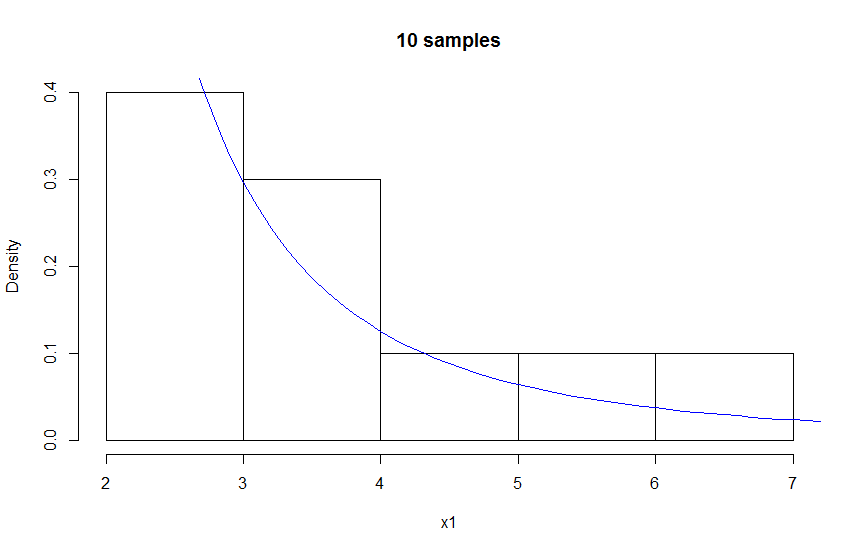
\includegraphics[width=10cm]{10Pareto.png}
				\caption{Pareto (2, 2) distribution, sampled 10 times}
			\end{figure}
			
			\begin{figure}[ht]
				\centering
				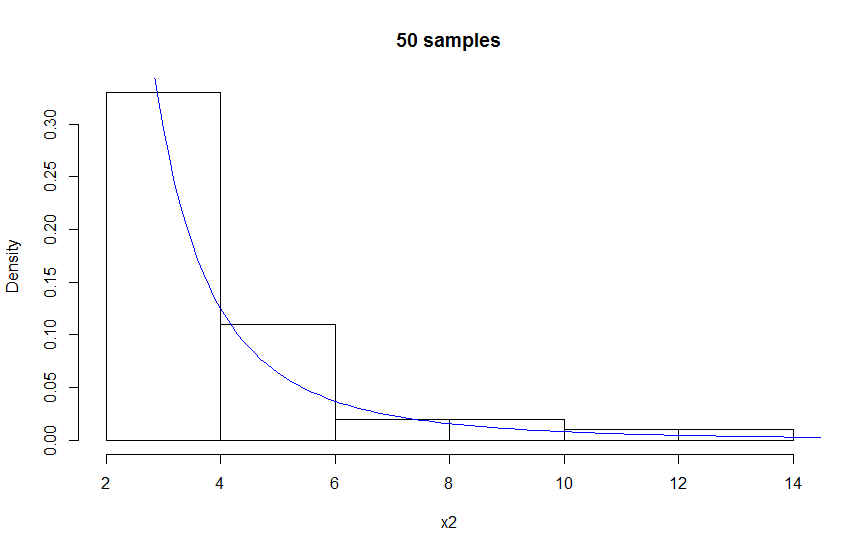
\includegraphics[width=10cm]{50Pareto.png}
				\caption{Pareto (2, 2) distribution, sampled 50 times}
			\end{figure}
			
			\begin{figure}[ht]
				\centering
				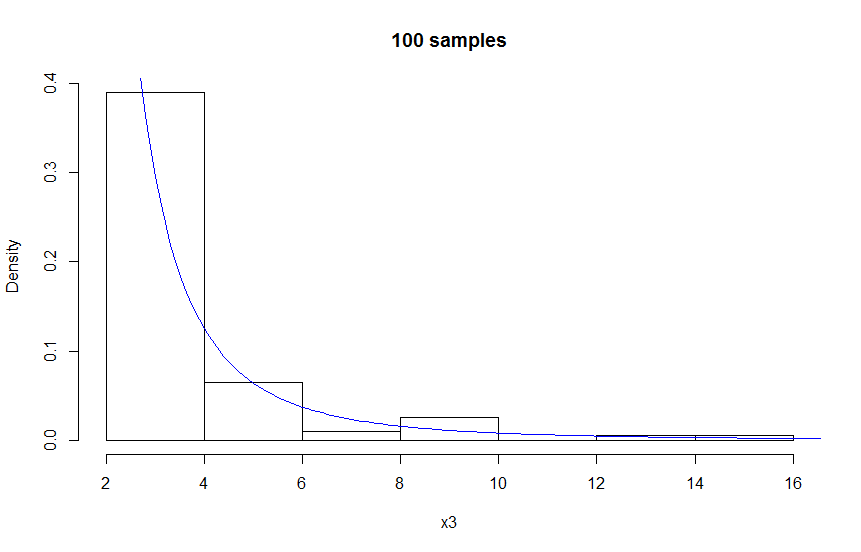
\includegraphics[width=10cm]{100pareto.png}
				\caption{Pareto (2, 2) distribution, sampled 100 times}
			\end{figure}
			
		\end{soln}
		
\end{enumerate}

\end{document}
